\documentclass[10pt,a4paper]{amsart}
\usepackage[margin=19mm]{geometry}
\usepackage{amsmath,amssymb,mathtools}
\usepackage[scr=rsfs,cal=euler]{mathalfa}
\usepackage{xfrac}
\usepackage[unicode,hidelinks,bookmarks=false]{hyperref}
\newcommand{\ie}{i.e.\ }
\newcommand{\cf}{cf.\ }
\newcommand{\resp}{respectively\ }
\newcommand{\Subsection}{\subsection}
\providecommand{\nobreakdash}{\nobreak\hbox{-}}
\setlength{\emergencystretch}{2em}
\multlinegap0pt
\usepackage{mathrsfs}
\usepackage{booktabs}
\usepackage{array}
\usepackage{longtable}
\usepackage{tikz}
\usepackage{lmodern}
\newtheorem{theorem}{Theorem}[section]
\newtheorem{lemma}[theorem]{Lemma}
\newtheorem{definition}[theorem]{Definition}
\newtheorem{remark}[theorem]{Remark}
\renewcommand{\Re}{\operatorname{Re}}
\begin{document}
\title[Radii of Concavity for Subclasses of Univalent Functions Ass]{Radii of Concavity for Subclasses of Univalent Functions Associated with the Exponential Mapping}
\author{Pradip Das; Nabadwip Sarkar}
\date{}
\maketitle
\noindent\emph{Source and licence.} Radii of Concavity for Subclasses of Univalent Functions Associated with the Exponential Mapping. Version arXiv:2609.26154v1 (CC BY 4.0). This material is distributed under the Creative Commons Attribution 4.0 International licence, http://creativecommons.org/licenses/by/4.0/, as recorded in the arXiv OAI licence metadata for this exact version and shown on the abstract page https://arxiv.org/abs/2609.26154v1. Full rights notice: licenses/arxiv-2609.26154-CC-BY-4.0.txt.\par\smallskip
\noindent\textit{Editorial scope.} Counted unit: the original \texttt{theorem} environment \texttt{T1} at source lines 398--409 together with its complete proof at lines 410--704; the delivered document keeps source lines 234--705 so that every referenced label and every citation resolves inside it. Native editable source is the paper's own concatenated TeX; the AMS wrapper is editorial formatting only. No publisher class, upstream script or unrelated artwork is redistributed.
\begin{equation}\label{pm1}
T_f(z)
=
\frac{2}{A-1}
\left[
\frac{A+1}{2}
\left(
\frac{1+z}{1-z}
\right)
-
1
-
\frac{zf''(z)}{f'(z)}
\right].
\end{equation}
The M\"obius factor
\[
\frac{1+z}{1-z}
\]
reflects the pole behavior at the boundary point $z=1$ and plays a fundamental role in the geometry of concave mappings.

The investigation of geometric radii constitutes a classical theme in geometric function theory \cite{pm8, pm9, pm12}. In particular, radius problems for subclasses associated with Ma--Minda differential subordinations have attracted considerable attention in recent years. However, to the best of our knowledge, radii of concavity associated with exponential Ma--Minda subclasses have not previously been studied within the Avkhadiev--Wirths framework.

Our primary objective is to determine the sharp radii of concavity for the classes $\mathcal{S}_e^*$ and $\mathcal{C}_e$ with respect to $\mathcal{C}_c(A)$. The resulting radii are characterized by explicit transcendental equations, and sharpness is established globally through extremal functions generated by the disk automorphism $\omega_0(z)=-z$.
\subsection{Radius of Concavity}

A distinctive feature of the class $\mathcal{C}_c(A)$ is that the defining geometric property is generally non-hereditary under dilations \cite{pm7}. Specifically, if
\[
f\in\mathcal{C}_c(A),
\]
the scaled function
\[
g(z)=r^{-1}f(rz)
\]
need not remain in $\mathcal{C}_c(A)$ for arbitrary $r\in(0,1]$. This naturally leads to the notion of the radius of concavity.

Following Bhowmik and Biswas \cite{pm7}, we adopt the following definition.

\begin{definition}
Let $\mathcal{F}\subset\mathcal{A}$. The radius of concavity of $\mathcal{F}$ with respect to the class $\mathcal{C}_c(A)$ is the largest number
\[
R_{\mathcal{F},\mathcal{C}_c(A)}\in(0,1]
\]
such that
\begin{equation}\label{pm2}
\Re\{T_f(z)\}>0
\qquad
\text{for all }
|z|<R_{\mathcal{F},\mathcal{C}_c(A)}
\end{equation}
and every function $f\in\mathcal{F}$.
\end{definition}

\begin{figure}[h!]
\centering
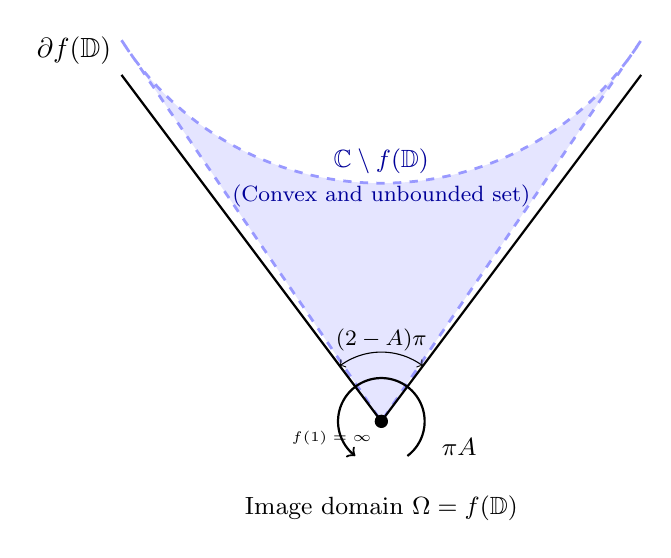
\begin{tikzpicture}[scale=2.2]

    % Complementary domain
    \draw[
        fill=blue!10,
        draw=blue!40,
        dashed,
        line width=1pt
    ]
    (-1.5,1.8)
    -- (0,-0.4)
    -- (1.5,1.8)
    .. controls (0.8,0.7) and (-0.8,0.7) ..
    (-1.5,1.8);

    % Boundary rays
    \draw[thick]
        (0,-0.4) -- (-1.5,1.6)
        node[above left] {$\partial f(\mathbb{D})$};

    \draw[thick]
        (0,-0.4) -- (1.5,1.6);

    % Exterior angle
    \draw[->, thick, domain=-53:233, samples=100]
        plot ({0.25*cos(\x)}, {-0.4 + 0.25*sin(\x)});

    \node at (0.45,-0.55)
        {\small $\pi A$};

    % Interior angle
    \draw[<->, thin, domain=53:127]
        plot ({0.4*cos(\x)}, {-0.4 + 0.4*sin(\x)});

    \node[above,font=\footnotesize]
        at (0,-0.05)
        {$(2-A)\pi$};

    % Labels
    \node[font=\small,text=blue!60!black]
        at (0,1.1)
        {$\mathbb{C}\setminus f(\mathbb{D})$};

    \node[font=\footnotesize,text=blue!60!black]
        at (0,0.9)
        {(Convex and unbounded set)};

    \node[font=\small]
        at (0,-0.9)
        {Image domain $\Omega=f(\mathbb{D})$};

    % Vertex
    \filldraw[black]
        (0,-0.4) circle (1pt);

    \node[below left,font=\tiny]
        at (0,-0.4)
        {$f(1)=\infty$};

\end{tikzpicture}

\caption{
Boundary geometry of a concave domain associated with
$f\in\mathcal{C}_c(A)$.
}

\label{fig:conformal_concave_wedge}
\end{figure}

Geometrically, the condition
\[
\Re\{T_f(z)\}>0
\]
ensures that the image of the subdisk
\[
\mathbb{D}_r=\{z\in\mathbb{C}:|z|<r\}
\]
under $f$ satisfies the concavity constraint determined by the opening angle parameter $\pi A$ \cite{pm6}. The present paper establishes the exact concavity radii for the exponential subclasses $\mathcal{S}_e^*$ and $\mathcal{C}_e$ within this framework.
\section{Auxiliary Lemmas}

\begin{lemma}[\cite{Mendiratta2015}]
\label{L2}
Let $\omega \in \Omega$. For $|z| = r < 1$, 
\[
e^{-r} \le \left| e^{\omega(z)} \right| \le e^r,
\]
and
\[
\Re\left(e^{\omega(z)}\right) \ge e^{-r}\cos(r).
\]
\end{lemma}

To analyze the combined variation of a Schwarz function and its derivative, we rely on the region of variability established by Dieudonn\'{e} \cite{Dieudonn\'e1931}.

\begin{lemma}[Dieudonn\'{e}'s Lemma \cite{Dieudonn\'e1931, pm8}]
\label{L3}
Let $\omega \in \Omega$. For a fixed point $z \in \mathbb{D}$ with $|z|=r$, the joint region of variability for the pair $(\omega(z), \omega'(z))$ is characterized by the inequality
\begin{equation}\label{eq:Dieudonn\'e1}
\left| z\omega'(z) - \omega(z) \right| \le \frac{r^2 - |\omega(z)|^2}{1 - r^2}.
\end{equation}
Equivalently, for a fixed value $\omega(z) = u+iv$, the value $z\omega'(z)$ lies in the closed disk
\begin{equation}\label{eq:Dieudonn\'e2}
\left| z\omega'(z) - (u+iv) \right| \le \frac{r^2 - (u^2+v^2)}{1 - r^2}.
\end{equation}
\end{lemma}


\section{Main Results}


\begin{theorem}[Radius of Concavity for the Class $\mathcal{S}_e^*$]
\label{T1}
Let $A\in(1,2]$. If a function $f\in\mathcal{S}_e^*$, then
\begin{equation}\label{operator_inequality}
\Re\{T_f(z)\}>0 \qquad \text{for } |z|<R_{\mathcal{S}_e^*,\mathcal{C}_c(A)},
\end{equation}
where $R_{\mathcal{S}_e^*,\mathcal{C}_c(A)}$ is the unique root in $(0,1)$ of the transcendental equation
\begin{equation}\label{pm3}
\Phi_1(r) := \frac{A+1}{2} \left( \frac{1-r}{1+r} \right) - e^r - r = 0.
\end{equation}
This radius threshold is sharp.
\end{theorem}

\begin{proof}
Since $f\in\mathcal{S}_e^*$, there exists a Schwarz function $\omega\in\Omega$ such that
\begin{equation}\label{pm4}
\frac{zf'(z)}{f(z)} = e^{\omega(z)}, \qquad z\in\mathbb{D}.
\end{equation}
Differentiating logarithmically gives
\begin{equation}\label{pm5}
1+\frac{zf''(z)}{f'(z)}
=
e^{\omega(z)}+z\omega'(z).
\end{equation}
Substituting \eqref{pm5} into the Avkhadiev--Wirths operator \eqref{pm1}, we obtain
\begin{equation}\label{pm6}
T_f(z)
=
\frac{2}{A-1}
\left[
\frac{A+1}{2}\left(\frac{1+z}{1-z}\right)
-
\left(e^{\omega(z)}+z\omega'(z)\right)
\right].
\end{equation}
Taking real parts yields
\begin{equation}\label{pm7}
\Re\{T_f(z)\}
=
\frac{2}{A-1}
\left[
\frac{A+1}{2}
\Re\left(\frac{1+z}{1-z}\right)
-
\Re\left(e^{\omega(z)}+z\omega'(z)\right)
\right].
\end{equation}

For $|z|=r<1$, the sharp M\"obius estimate
\[
\Re\left(\frac{1+z}{1-z}\right)
\ge
\frac{1-r}{1+r}
\]
implies
\begin{equation}\label{pm8}
\Re\{T_f(z)\}
\ge
\frac{2}{A-1}
\left[
\frac{A+1}{2}\left(\frac{1-r}{1+r}\right)
-
\Re\left(e^{\omega(z)}+z\omega'(z)\right)
\right].
\end{equation}

We now maximize the quantity
\[
\Re\left(e^{\omega(z)}+z\omega'(z)\right).
\]
Fix $z\in\mathbb{D}$ with $|z|=r$, and write
\[
\omega(z)=u+iv.
\]
By Dieudonn\'es lemma,
\begin{equation}\label{pm9}
\left|
z\omega'(z)-(u+iv)
\right|
\le
\frac{r^2-(u^2+v^2)}{1-r^2}.
\end{equation}
Note that $\Re(z\omega')=u+\Re(z\omega'-\omega)$ and $\Re(z\omega'-(u+iv))\leq |z\omega'-(u+iv)|$.
Hence
\begin{equation}\label{pm10}
\Re\left(e^{\omega(z)}+z\omega'(z)\right)
\le \Re\left(e^{\omega(z)}\right)+\Re\left(z\omega'(z)\right)\leq
e^u\cos v
+
u
+
\frac{r^2-u^2-v^2}{1-r^2}.
\end{equation}

Define
\begin{equation}\label{pm_psi_def}
\Psi(u,v)
=
e^u\cos v
+
u
+
\frac{r^2-u^2-v^2}{1-r^2},
\qquad
u^2+v^2\le r^2.
\end{equation}
Differentiating with respect to $v$ gives
\[
\frac{\partial\Psi}{\partial v}
=
-e^u\sin v
-
\frac{2v}{1-r^2}.
\]
Thus
\[
\frac{\partial\Psi}{\partial v}<0
\qquad
(1>r\geq v>0),
\]
and by symmetry the maximum occurs at $v=0$. Therefore the problem reduces to maximizing
\begin{equation}\label{pm_psi_u_def}
\psi(u)
=
e^u
+
u
+
\frac{r^2-u^2}{1-r^2},
\qquad
u\in[-r,r].
\end{equation}
Differentiation yields
\begin{equation}\label{pm_psi_prime}
\psi'(u)
=
e^u
+
1
-
\frac{2u}{1-r^2}.
\end{equation}

Next, observe that
\[
\Phi_1(r)
\le
\frac{3}{2}\left(\frac{1-r}{1+r}\right)-e^r-r.
\]
Since
\[
\frac{3}{2}\left(\frac{1-0.25}{1+0.25}\right)
-e^{0.25}
-0.25
<0,
\]
the unique root of $\Phi_1(r)=0$ satisfies
\[
R_{\mathcal S_e^*,\mathcal C_c(A)}<0.25
\]
for all $A\in(1,2]$.

Consequently, for $0<r<0.25$ and $u\in[-r,r]$,
\[
e^u\ge e^{-0.25},
\qquad
-\frac{2u}{1-r^2}
\ge
-\frac{0.5}{1-0.25^2}.
\]
Hence
\[
\psi'(u)
>
e^{-0.25}
+
1
-
\frac{0.5}{1-0.25^2}
>
0.
\]
Therefore $\psi(u)$ is strictly increasing on $[-r,r]$, and its maximum occurs at $u=r$. Substituting into \eqref{pm_psi_u_def} gives
\begin{equation}\label{pm11}
\max_{-r\le u\le r}\psi(u)
=
\psi(r)
=
e^r+r.
\end{equation}

Combining \eqref{pm8} and \eqref{pm11}, we obtain
\[
\Re\{T_f(z)\}
\ge
\frac{2}{A-1}
\left[
\frac{A+1}{2}\left(\frac{1-r}{1+r}\right)
-
(e^r+r)
\right]
=
\frac{2}{A-1}\Phi_1(r).
\]
Thus
\[
\Re\{T_f(z)\}>0
\]
whenever $\Phi_1(r)>0$.

We now prove existence and uniqueness of the root of $\Phi_1$. Since
\[
\Phi_1(0)=\frac{A-1}{2}>0,
\]
and
\[
\lim_{r\to1^-}\Phi_1(r)=-(e+1)<0,
\]
the Intermediate Value Theorem guarantees at least one root in $(0,1)$.

Differentiating,
\begin{equation}\label{pm_phi_prime}
\Phi_1'(r)
=
-\frac{A+1}{(1+r)^2}
-
e^r
-
1
<
0.
\end{equation}
Hence $\Phi_1$ is strictly decreasing on $(0,1)$, and the root is unique.

To prove sharpness, define
\begin{equation}\label{eq:extremal_f0}
f_0(z)
=
z\exp\left(
\int_0^z
\frac{e^{-t}-1}{t}\,dt
\right).
\end{equation}
Then
\[
\frac{zf_0'(z)}{f_0(z)}
=
e^{-z},
\]
so $f_0\in\mathcal S_e^*$ with extremal Schwarz function $\omega_0(z)=-z$.

Moreover,
\[
\Re\left\{
\frac{zf_0'(z)}{f_0(z)}
\right\}
=
e^{-x}\cos y>0
\qquad
(z=x+iy\in\mathbb D),
\]
since $|y|<1$. Hence $f_0$ is starlike and therefore univalent.

Differentiating once more yields
\[
1+\frac{zf_0''(z)}{f_0'(z)}
=
e^{-z}-z.
\]
Substituting into \eqref{pm1}, we obtain
\[
T_{f_0}(z)
=
\frac{2}{A-1}
\left[
\frac{A+1}{2}\left(\frac{1+z}{1-z}\right)
-
(e^{-z}-z)
\right].
\]
Evaluating at $z=-r$ gives
\[
T_{f_0}(-r)
=
\frac{2}{A-1}\Phi_1(r).
\]
Hence
\[
\Re\{T_{f_0}(-r)\}<0
\qquad
(r>R_{\mathcal S_e^*,\mathcal C_c(A)}),
\]
showing that the radius cannot be improved.

Finally, for the extremal choice $\omega_0(z)=-z$,
\[
|z\omega_0'(z)-\omega_0(z)|=0,
\]
and equality is attained simultaneously in all optimization steps, including
\[
\Re(e^{\omega_0(z)})
=
e^u\cos(0)
=
e^u.
\]
Therefore the radius is sharp.
\end{proof}

\begin{thebibliography}{99}
\bibitem[Dieudonn\'e1931]{Dieudonn\'e1931} J.~Dieudonn\'e, Recherches sur quelques probl\`emes relatifs aux polyn\^omes et aux fonctions born\'ees d'une variable complexe, \emph{Ann. Sci. \'Ec. Norm. Sup\'er.} \textbf{48} (1931), 247--358.
\bibitem[Mendiratta2015]{Mendiratta2015} R.~Mendiratta, S.~Nagpal, and V.~Ravichandran, On a subclass of strongly starlike functions associated with exponential function, \emph{Bull. Malays. Math. Sci. Soc.} \textbf{38} (2015), no.~1, 365--386.
\bibitem[pm12]{pm12} T.~H.~MacGregor, Functions whose derivative has a positive real part, \emph{Trans. Amer. Math. Soc.} \textbf{104} (1962), no.~3, 532--537.
\bibitem[pm6]{pm6} F.~G.~Avkhadiev and K.-J.~Wirths, Concave schlicht functions with bounded opening angle at infinity, \emph{Lobachevsky J. Math.} \textbf{17} (2005), 3--10.
\bibitem[pm7]{pm7} B.~Bhowmik and S.~Biswas, Distortion, radius of concavity and several other radii results for certain classes of functions, \emph{Comput. Methods Funct. Theory} \textbf{24} (2024), no.~2, 525--538.
\bibitem[pm8]{pm8} P.~L.~Duren, \emph{Univalent Functions}, Springer-Verlag, New York, 1983.
\bibitem[pm9]{pm9} T.~H.~MacGregor, The univalence of a linear combination of convex mappings, \emph{J. London Math. Soc.} \textbf{44} (1969), no.~1, 210--212.
\end{thebibliography}
\end{document}
